% 2011 年江西卷理科第 21 题：四面体 A1A2A3A4。
% 来源 PDF：普通高考/2011/2011江西理.pdf，SHA-256 9fa84ea67ec469ea2a8bb4a06f9d79b6c5a94e8b08a52d2045e30daabf8d1582。
% 原页：第 2 页第 3 栏，书页码 678。
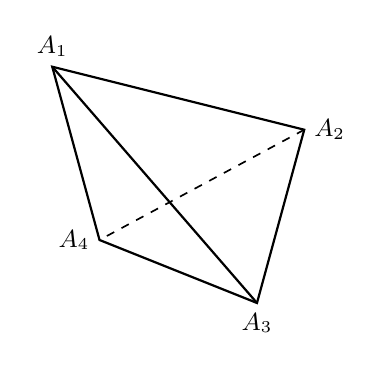
\begin{tikzpicture}[>=stealth, semithick, font=\small, scale=1.0]
  \coordinate (A1) at (0,3.0);
  \coordinate (A2) at (3.2,2.2);
  \coordinate (A3) at (2.6,0);
  \coordinate (A4) at (0.6,0.8);
  \draw[thick] (A1)--(A2)--(A3)--(A4)--cycle;
  \draw[thick] (A1)--(A3);
  \draw[dashed] (A2)--(A4);
  \node[above] at (A1) {$A_1$};
  \node[right] at (A2) {$A_2$};
  \node[below] at (A3) {$A_3$};
  \node[left] at (A4) {$A_4$};
\end{tikzpicture}
